\documentclass[aspectratio=1610,handout]{beamer}
\usepackage[utf8]{inputenc}
\usepackage{booktabs}
\usepackage{tabulary}
\usepackage{amssymb}% http://ctan.org/pkg/amssymb
\usepackage{pifont}% http://ctan.org/pkg/pifont
\usepackage{csquotes}
\usepackage{booktabs}
\usepackage{tikz}
\usetikzlibrary{arrows.meta,positioning,quotes}
\definecolor{darkred}{RGB}{200,50,50}
\usepackage{aurl}
\daurl{hito}{http://hitontology.eu/ontology/}
\daurl{}{http://hitontology.eu/ontology/}
\newcommand{\cmark}{\ding{51}}%
\newcommand{\xmark}{\ding{55}}%
\newcommand{\both}[1]{{\color[rgb]{0.8,1,0.8}\textbf{#1}}}
\newcommand{\onlyone}[1]{{\color[rgb]{1,0.4,0.4}\textbf{#1}}}
\newcommand{\K}[1]{\textnormal{K}{(#1)}}
\newcommand{\E}[1]{\textnormal{E}{(#1)}}
\newcommand{\D}[1]{\textnormal{E}{(#1)}}
\newcommand{\f}[1]{\ensuremath{f(#1)}}
\newcommand{\fl}[1]{\ensuremath{f_{\lambda}(#1)}}
\usetheme{simple}
\usecolortheme{whiteonblack}

%\title{Semantische Ähnlichkeit von HITO Softwareprodukten}
\title{Clustern von HITO-Softwareprodukten}
%\subtitle{Automatisches Finden von Gemeinsamkeiten und Untersc}
%\author{Konrad Höffner}
\date{9. September 2021}

% Parameters: frame title, image path, (optional) note
\newcommand{\imageslide}[4][]
{
%\newgeometry{margin=0.0cm,top=1em}
\begin{frame}[plain]{~~~~#2}
\vspace{0.2em}
\begin{center}
\centering\includegraphics[width=1.0\textwidth,height=0.9\textheight,keepaspectratio]{#3}
\end{center}
#1
\note{#4}
\end{frame}
%\restoregeometry
}

% https://tex.stackexchange.com/questions/9681/how-to-draw-venn-diagrams-especially-complements-in-latex
\newcommand{\intersection}[1]
{
\begin{tikzpicture}[fill=darkred]
% left hand
\scope
\clip (-2,-2) rectangle (3,2)
      (#1,0) circle (1);
\fill (0,0) circle (1);
\endscope
% right hand
\scope
\clip (-2,-2) rectangle (3,2)
      (0,0) circle (1);
\fill (#1,0) circle (1);
\fill (#1,0) circle (1);
\endscope
% outline
\draw (0,0) circle (1) (0,1)  node [text=black,above] {$A$}
      (#1,0) circle (1) (#1,1)  node [text=black,above] {$B$}
      (-2,-2) rectangle (3,2) node [text=black,above] {$H$};
\end{tikzpicture}
}


\begin{document}
\begin{frame}
\titlepage
\end{frame}


\imageslide{Softwareprodukte und Umgebung}{img/snik-graph.jpg}{\tiny\url{https://www.snik.eu/pgraph/?sparql=https://hitontology.eu/sparql&graph=http://hitontology.eu/ontology&instances}}

\imageslide{Softwareprodukte und Umgebung}{img/hito-labelled.jpg}{\tiny\url{https://www.snik.eu/pgraph/?sparql=https://hitontology.eu/sparql&graph=http://hitontology.eu/ontology&instances}}

\begin{frame}{Problem}
\begin{itemize}
\item viel Wissen über SWPs gesammelt, was können wir daraus ableiten?
\item Tools wie LodView zeigen Details über einzelne SWPs aber SNIK Graph bietet keinen guten Gesamtüberblick
\item Anwendungsystemtypen (ASTs) bieten manuelle Gruppierung aber wie ähnlich sind deren Produkte wirklich?
\item Gibt es ähnliche SWPs in unterschiedlichen ASTs?
\item Können wir neue ASTs finden?
%\item Kombination von Eigenschaften zu einem Maß für die Distanz oder Ähnlichkeit zwischen zwei Softwareprodukten
%\item wichtige Eigenschaften sind unbekannt
%\item Exploratives Data Mining: Finden eines solchen Maßes
\end{itemize}
\end{frame}

\begin{frame}{TODO: Clustering nach Anwendungssystemtypen hier einfügen}
\end{frame}

\begin{frame}{Preprocessing}
Abbilden von SWPs auf direkte Nachbarschaft (siehe Anhang NSWD):
\begin{align*}
V_{in}(x)	&= \{v \in I| \langle v,p,x \rangle \in \textnormal{KB}\}\\
V_{out}(x)	&= \{v \in I| \langle x,p,v \rangle \in \textnormal{KB}\}\\
V_{all}(x)	&= V_{in}(x) \cup V_{out}(x)
\end{align*}

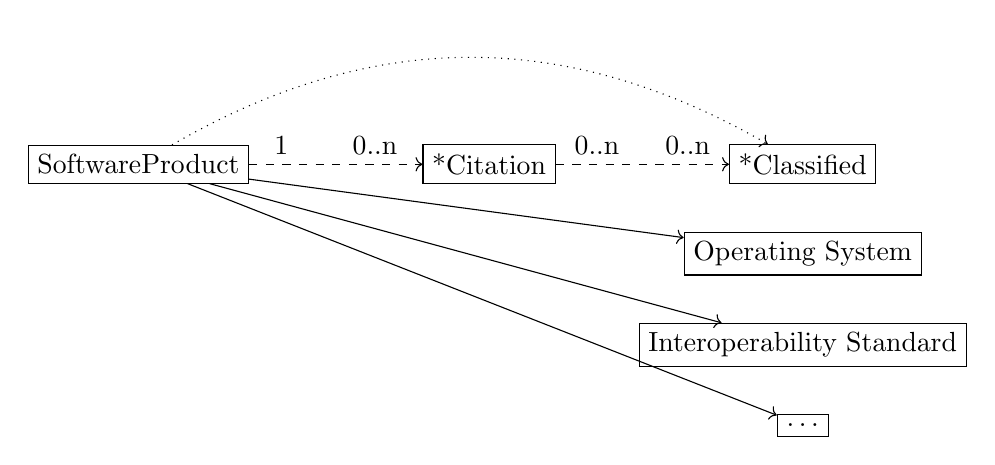
\begin{tikzpicture}[auto,box/.style={draw},node distance = 6mm and 22mm,->]
\node (n1) [box] {SoftwareProduct};
\node (n2) [box] [right=of n1]{*Citation};
\node (n3) [box] [right=of n2]{*Classified};
\node (n4) [box] [below=of n3]{Operating System};
\node (n5) [box] [below=of n4]{Interoperability Standard};
\node (n6) [box] [below=of n5]{$\ldots$};

\draw	(n1) edge ["1~~~~~~~0..n",dashed] (n2)
	(n2) edge ["0..n~~~~~0..n",dashed] (n3)
	(n1) edge [bend left,dotted] (n3)
	(n1) edge (n4)
	(n1) edge (n5)
	(n1) edge (n6);
\end{tikzpicture}

\end{frame}

\begin{frame}{Tele DICOM vs Cerner FirstNet}
\textbf{\aurl{}{TeleDicom}}\\
\onlyone{
\aurl{}{EhrSfmManageResults}\\
\aurl{}{EhrSfmManageResultsOfDiagnosticTests}
\aurl{}{EhrSfmSupportForCommunicationsBetweenOrganizations}
\aurl{}{EhrSfmSupportRemoteHealthcareServices}
}
~\\~\\
\textbf{\aurl{}{CernerFirstNet}}\\
\onlyone{
\aurl{}{EhrSfmManageCareCoordinationReporting}
\aurl{}{EhrSfmManageClinicalDocumentation}
\aurl{}{EhrSfmManageHealthcareResourceScheduling}
\aurl{}{EhrSfmProduceASummaryRecordOfCare}
\aurl{}{EhrSfmSupportCareCoordinationReporting}
\aurl{}{EhrSfmSupportTriageCategorization}\\
}
~\\
Keine gemeinsamen Eigenschaften, sehr unterschiedlich?
\end{frame}

\begin{frame}{Ris1 vs Ris2---Ris1}
\both{
BbAdministrativeDischargeAndBilling
BbArchivingOfPatientInformation
BbControlling}
\onlyone{
BbInformationManagement
BbLongTermArchiving
BbOrderEntry}
\both{
BbPatientAdministration
BbPatientAdmission
BbQualityManagement
BbSchedulingAndResourceAllocation
}
\onlyone{
BbSupplyAndDisposalManagement
C++
C\_Sharp}
\both{
DICOM
}
\onlyone{
English
GDT
}
\both{
German
HL7
}
\onlyone{
Linux
Macintosh
Microsoft\_Windows
Unix
WebBased
}
\onlyone{WhoDhiAutomatedAnalysisOfDataToGenerateNewInformationOrPredictionsOnFutureEvents}
\both{WhoDhiDataExchangeAcrossSystems}
\onlyone{WhoDhiDataExchangeAndInteroperability
WhoDhiDataStorageAndAggregation
WhoDhiDataSynthesisAndVisualization}
\both{
WhoDhiEnrolClientForHealthServicesclinicalCarePlan
WhoDhiLongitudinalTrackingOfClientsHealthStatusAndServices
WhoDhiManageBudgetAndExpenditures}
\onlyone{
WhoDhiManageInventoryAndDistributionOfHealthCommoditiesStockLevelsOf
WhoDhiMapLocationOfHealthFacilitiesstructures
WhoDhiNonRoutineDataCollectionAndManagement
}
\both{WhoDhiTrackAndManageInsuranceReimbursement}
\onlyone{WhoDhiTransmitDiagnosticOrdersDiagnosticResults}
\end{frame}

\begin{frame}{Ris1 vs Ris2---Ris2}
\both{BbAdministrativeDischargeAndBilling}
\both{BbArchivingOfPatientInformation}
\both{BbControlling}
\both{BbPatientAdministration}
\both{BbPatientAdmission}
\both{BbQualityManagement}
\both{BbSchedulingAndResourceAllocation}
\both{DICOM}
\both{German}
\both{HL7}
\onlyone{Java}
\onlyone{JHTML}
\both{WebBased}
\both{WhoDhiDataExchangeAcrossSystems}
\both{WhoDhiEnrolClientForHealthServicesclinicalCarePlan}
\both{WhoDhiLongitudinalTrackingOfClientsHealthStatusAndServices}
\both{WhoDhiManageBudgetAndExpenditures}
\both{WhoDhiTrackAndManageInsuranceReimbursement}
\onlyone{Windows\_7}
\onlyone{Windows\_Vista}
\end{frame}

\begin{frame}{Übereinstimmung von Mengen}
\begin{itemize}
\item gesucht: $s: S \times S \rightarrow  \mathbb{R}, S = 2^E$
\item Ähnlichkeit $\leftrightarrow$ Distanz
\pause
\item Ähnlichkeit als Größe der Schnittmenge $|A \cap B|$
\pause
\item Jaccard-Koeffizient \[J(A,B) = \frac{|A \cap B|}{|A \cup B|}\]
\end{itemize}
\begin{center}
\intersection{0.5}
\intersection{1.5}
\end{center}
\end{frame}

%SELECT ?class (COUNT(?instance) AS ?count)
%{
% ?class a owl:Class.
% ?instance a ?class.
% FILTER EXISTS {?s a hito:SoftwareProduct. {?s ?p ?instance.} UNION {?s ?p [?q ?instance]}}
%} ORDER BY DESC(?count)

\begin{frame}{Alternative: Modellierung als Vektor}
\begin{tabular}{lll}
\toprule
Classified / Attribut		&ingesamt	&benutzt\\
\midrule
Feature						&619		&245\\
Function					&85			&49\\	
Interoperability			&104		&20\\
Operating System			&97			&20\\
Application System			&51			&10\\
Programming Library			&50			&3\\
User Group					&45			&8\\
\ldots\\
\midrule
$\Sigma$					&			&403\\
\bottomrule
\end{tabular}
~\\~\\
Jedes Feature, Function (classified), jede Sprache$\ldots$ ist eine eigene Dimension.\\
\end{frame}

\begin{frame}{Modellierung als Vektor---Fiktives Beispiel}
Labels sind kategorische (qualitative) Variablen. Umwandeln in quantitative Daten mit Python Bibliothek scikit learn DictVectorizer: one-hot encoding
\begin{columns}
 
 \begin{column}{.4\textwidth}
   \[\left(\begin{array}{c} \textnormal{Archive Pictures} \\ \textnormal{Admit Patients} \\ \textnormal{English} \\ \textnormal{Java} \\ \textnormal{Decision Support System} \\ \textnormal{RIS} \\ \textnormal{PACS} \\ \dots \\ \\ \\ \\ \\ \end{array}\right) \]
 \end{column}
 
 \begin{column}{.25\textwidth}
   \[\vec{GnuHealth}	= \left(\begin{array}{c} 0 \\ 0 \\ 0 \\ \both{1} \\ 0 \\ 0 \\ 1 \\ 0 \\ 0 \\ 0 \\ \ldots \\ 0 \\ 1 \end{array}\right) \]
 \end{column}

 \begin{column}{.25\textwidth}
   \[\vec{Bahmni}		= \left(\begin{array}{c} 1 \\ 0 \\ 0 \\ \both{1} \\ 0 \\ 0 \\ 0 \\ 0 \\ 0 \\ 0 \\ \ldots \\ 0 \\ 0 \end{array}\right) \]
 \end{column}
\end{columns}

\end{frame}

\begin{frame}{Dimensionsreduzierung und Clustering}
\begin{itemize}
\item Principal Component Analysis (PCA)
\item Affinity Propagation clustering
\end{itemize}
\end{frame}

\imageslide{HITO l1 norm}{img/cluster-l1.pdf}{}
\imageslide{HITO l1 norm classified only}{img/cluster-classifiedonly-l1.pdf}{}
\imageslide{HITO l2 norm}{img/cluster-l2.pdf}{}
\imageslide{HITO l2 norm classified only}{img/cluster-classifiedonly-l2.pdf}{}
\imageslide{HITO max norm}{img/cluster-max.pdf}{}
\imageslide{HITO max norm classified only}{img/cluster-classifiedonly-max.pdf}{}


\begin{frame}{Alternative: Bag of Words}
\begin{itemize}
\item bag: Menge mit Mehrfachvorkommen
\item Zusammenfügen der Labels aller Eigenschaften
\item CountVectorizer
\item PCA, Affinity Propagation Clustering
\end{itemize}
\end{frame}

\begin{frame}{Bag of Words---Beispiel, classified only}
\small
\textbf{Ris1} Administrative discharge and billing Archiving of patient information Automated analysis of data to generate new information or predictions on future events Controlling Data exchange across systems Data exchange and interoperability Data storage and aggregation Data synthesis and visualization Enrol client for health services/clinical care plan Longitudinal tracking of client’s health status and services received Manage budget and expenditures Manage inventory and distribution of health commodities Map location of health facilities/structures Non routine data collection and management Order entry Quality management Scheduling and resource allocation Supply and disposal management Track and manage insurance reimbursement Transmit and track diagnostic orders information management long term archiving patient administration patient admission
\\~\\
\textbf{Ris2} Administrative discharge and billing Archiving of patient information Controlling Data exchange across systems Enrol client for health services/clinical care plan Longitudinal tracking of client’s health status and services received Manage budget and expenditures Quality management Scheduling and resource allocation Track and manage insurance reimbursement patient administration patient admission
\end{frame}

\imageslide{HITO BOW l1 norm}{img/cluster-bagofwords-l1.pdf}{}
\imageslide{HITO BOW l1 norm classified only}{img/cluster-bagofwords-classifiedonly-l1.pdf}{}
\imageslide{HITO BOW l2 norm}{img/cluster-bagofwords-l2.pdf}{}
\imageslide{HITO BOW l2 norm classified only}{img/cluster-bagofwords-classifiedonly-l2.pdf}{}
\imageslide{HITO BOW max norm}{img/cluster-bagofwords-max.pdf}{}
\imageslide{HITO BOW max norm classified only}{img/cluster-bagofwords-classifiedonly-max.pdf}{}

\begin{frame}{UMAP---Uniform Manifold Approximation and Projection for Dimension Reduction}
\begin{itemize}
\item Alternative zu PCA
\item Hyperparameter n\_neighbours bestimmt lokale vs globale Struktur
\end{itemize}
\end{frame}

\imageslide{HITO BOW max norm classified only UMAP neighbours=5}{img/cluster-bagofwords-classifiedonly-umap-n5-max.pdf}{}
\imageslide{HITO BOW max norm classified only UMAP neighbours=6}{img/cluster-bagofwords-classifiedonly-umap-n6-max.pdf}{}
\imageslide{HITO BOW max norm classified only UMAP neighbours=7}{img/cluster-bagofwords-classifiedonly-umap-n7-max.pdf}{}
\imageslide{HITO BOW max norm classified only UMAP neighbours=8}{img/cluster-bagofwords-classifiedonly-umap-n8-max.pdf}{}
\imageslide{HITO BOW max norm classified only UMAP neighbours=9}{img/cluster-bagofwords-classifiedonly-umap-n9-max.pdf}{}
\imageslide{HITO BOW max norm classified only UMAP neighbours=10}{img/cluster-bagofwords-classifiedonly-umap-n10-max.pdf}{}
\imageslide{HITO BOW max norm classified only UMAP neighbours=15}{img/cluster-bagofwords-classifiedonly-umap-max.pdf}{}
\imageslide{HITO BOW max norm classified only UMAP neighbours=100}{img/cluster-bagofwords-classifiedonly-umap-n100-max.pdf}{}

\begin{frame}{TODO / Future Work}
\begin{itemize}
\item Hierarchical Clustering
\item Application System Type (AST) vorhersagen
\item ASTs vergleichen
\item neue ASTs finden
\item Vergleich existierende ASTs mit gefundenen Clustern
\pause
\vspace{1em}
\item Welche Eigenschaften interessieren wen wie stark? Programmiersprache vs Feature.
\pause
\item Häufige Eigenschaften automatisch abschwächen?
\pause
\item Korrelationen einbeziehen? Microsoft\_Windows vs Windows\_7
\pause
\item Unterschiedliche Kataloge
\pause
\item Gruppieren von Eigenschaften?
\end{itemize}
\end{frame}

\begin{frame}{Fragen?}
\end{frame}

\section{Anhang---Reinnehmen oder aus Zeitgründen rauslassen}

\begin{frame}{Informationsgehalt---Kolmogorov-Komplexität}
\begin{itemize}
\item Maß für den Informationsgehalt einer Zeichenkette $x$
\item $\K{x}$ Länge des kürzesten Programms, das $x$ erzeugt
\item $\K{x|y}$ Länge des kürzesten Programms, das $y$ erzeugt bei Eingabe von $x$
\item nicht berechenbar
\end{itemize}
\end{frame}

\begin{frame}{Distanz und Metrik~\cite{normalizedinformationdistance}}
Distanzfunktion $D: X \times  X \rightarrow \mathbb{R}^+$\\
\pause
~\\
Metrik\\~\\
\begin{tabular}{lr}
$\D{x,y} = 0$ gdw. $x = y$			&Identität\\
$\D{x,y} = \D{y,x}$					&Symmetrie\\
$\D{x,z} \leq \D{x,y} + \D{y,z}$	&Dreiecksungleichung\\
\end{tabular}\\
\pause
~\\~\\Informationsdistanz
\[\E{x,y} = \max(\K{x|y},\K{y|x}) \approx K(xy) - \min(\K{x},\K{y}) \]
\pause
Normalized Information Distance NID\\
\[e(x,y) = \frac{\max(\K{x|y},\K{y|x})}{\max(\K{x},\K{y})} \]
\end{frame}

\begin{frame}{NWD---Normalized Web Distance}
\begin{itemize}
\item $N$ Webseiten
\item Suchmaschine G liefert $\f{x}$ Treffer bei Suche nach $x$
\end{itemize}
~\\
\[\textnormal{e}_G(x,y) = \frac
{\max(\log \f{x}, \log \f{y})- \log \f{x,y}}
{\log N - \min(\log \f{x}, \log \f{y})}
\]
\end{frame}

\begin{frame}{NSWD---Normalized Semantic Web Distance~\cite{normalizedsemanticwebdistance}}
\begin{align*}
V_{in}(x)	&= \{v \in I| \langle v,p,x \rangle \in \textnormal{KB}\}\\
V_{out}(x)	&= \{v \in I| \langle x,p,v \rangle \in \textnormal{KB}\}\\
V_{all}(x)	&= V_{in}(x) \cup V_{out}(x)
\end{align*}
\begin{align*}
\lambda		&\in \{\textnormal{in}, \textnormal{out}, \textnormal{all}\}\\
\f{x}		&= |V_{\lambda}(x)|\\
\f{x,y}	&= |V_{\lambda}(x) \cap V_{\lambda{y}}|
\end{align*}
\[
\textnormal{NSWD}_{\lambda}(x,y) = \frac{\max(\log \fl{x}, \log \fl{y})- \log \fl{x,y}}{\log N - \min(\log \fl{x}, \log \fl{y})}
\]
\end{frame}

\begin{frame}{NSWD---Adaptations to HITO}
\begin{itemize}
\item Citations werden nur einmal benutzt und tauchen daher nie in $\f{x,y}$ auf $\rightarrow$ ersetzen durch classifieds
%\item keine Überschneidung im Wertebereich der SWP-Properties $\rightarrow |\langle v,p,x \angle | = | v,x |$ 
\item Beschränkung auf $V_{out}$
\end{itemize}
\end{frame}

\begin{frame}{NSWD}
\begin{tabular}{llr}
CscMedChart					&CernerMilleniumPowerOrders	&0.0\\
GePatchspecdPacs					&AbbottIStat	&0.0\\
TeleDicom					&EChasqui	&0.0623\\
CernerSoarianCpoePlatform					&CernerMilleniumPowerOrders	&0.0683\\
CscMedChart					&CernerSoarianCpoePlatform	&0.0683\\
Theriak					&Medicator	&0.0798\\
Theriak					&CernerSoarianCpoePlatform	&0.1153\\
AgfaPacsImpax					&AbbottIStat	&0.1414\\
GePatchspecdPacs					&AgfaPacsImpax	&0.1414\\
Theriak					&CernerMilleniumPowerOrders	&0.1440\\
Theriak					&CscMedChart	&0.1440\\
AgfaRisElefante					&AbbottIStat	&0.1502\\
\end{tabular}\\
~\\Hier scheint ein Fehler in den Daten zu sein, Distanz 0 sollte eigentlich dort nicht sein, untersuchen.
\end{frame}

\begin{frame}{Referenzen}
\bibliographystyle{unsrt}
\bibliography{hitocluster}
\end{frame}

\end{document}
